%%%%%%%%%%%%%%%%%%%%%%%%%%%%%%%%%%%%%%%%%
% Original author:
% Adrien Friggeri (adrien@friggeri.net)
% https://github.com/afriggeri/CV
%
% Modified by:
% Nuno Lourenço (me@nunolourenco.me)


\documentclass[]{friggeri-cv} % Add 'print' as an option into the square bracket to remove colors from this template for printing
\usepackage{graphicx}

\addbibresource{bibliography.bib} % Specify the bibliography file to include publications

\begin{document}

\header{Nuno}{ Louren\c{c}o}{Ph.D. Researcher} % Your name and current job title/field

%----------------------------------------------------------------------------------------
%	SIDEBAR SECTION
%----------------------------------------------------------------------------------------

\begin{aside} % In the aside, each new line forces a line break
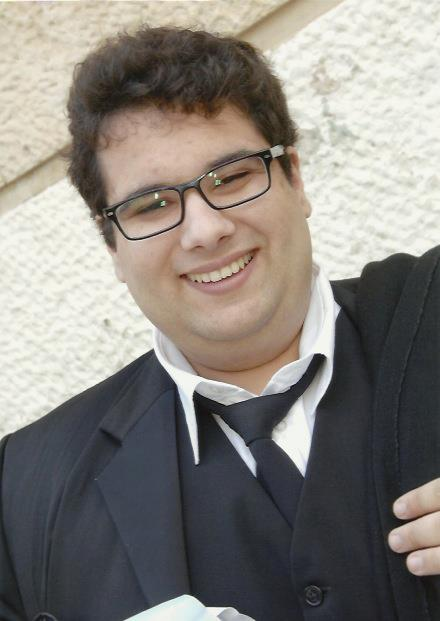
\includegraphics[scale=0.2]{me.jpeg}
\section{bio}
\textbf{Name}: Nuno António Marques Lourenço
\textbf{Birth}: November 14, 1988
\textbf{Citizenship}: Portuguese
\section{contact}
Rua do Pisão N.º 2, Foz de Arouce
3200-104 Lousã
Coimbra
Portugal
~
+351 914 544 370
~
\href{mailto:naml@dei.uc.pt}{naml@dei.uc.pt}
\href{mailto:me@nunolourenco.me}{me@nunolourenco.me}
\href{http://nunolourenco.me}{http://nunolourenco.me}
\section{languages}
Portuguese
English fluent
\section{programming}
Python, Java
C, C++
\section{research interests}
Hyper-Heuristics \\ {Evolutionary Computation} \\ Complex Systems \\ Artificial Intelligence \\ Problem Optimization \\ Machine Learning \\ Biology \\ Compilers
\end{aside}



%----------------------------------------------------------------------------------------
%	EDUCATION SECTION
%----------------------------------------------------------------------------------------


\section{Education}

\begin{entrylist}
%------------------------------------------------
\entry
{2011--\emph{Present}}
{Ph.D. {\normalfont candidate on Evolutionary Computation}}
{University of Coimbra, Portugal}
{Dissertation subject \emph{Evolution of Evolutionary Algorithms} under the guidance of the professors Ernesto Costa and Francisco B. Pereira }\\
%------------------------------------------------
\entrymasters
{2009--2011}
{Masters {\normalfont in Informatics Engineering}}
{University of Coimbra, Portugal}
{\emph{Swarm Intelligence Algorithms for Cluster Geometry Optimization} \\ This dissertation proposed an Ant Colony Optimization algorithm to tackle the problem of Cluster Geometry Optimization}
{\textbf{Advisors:} Dr. Francisco B. Pereira and Dr. Luís Paquete}
{\textbf{Thesis Grade:} 19/20}
{\textbf{Graduated} with 17/20}
%------------------------------------------------
\entry
{2006--2009}
{Bachelor {\normalfont in Informatics Engineering}}
{University of Coimbra, Portugal}
{\textbf{Graduated} with 16/20}
%------------------------------------------------
\end{entrylist}

%----------------------------------------------------------------------------------------
%	WORK EXPERIENCE SECTION
%----------------------------------------------------------------------------------------

\section{Teaching Experience}

\begin{entrylist}
%------------------------------------------------
\entry
{2011--2012}
{University of Coimbra}
{Coimbra, Portugal}
{\emph{Invited Assistant Professor} \\
Courses: \emph{Operating Systems} and \emph{Compilers}}
%------------------------------------------------
\entry
{2010-2011}
{University of Coimbra}
{Coimbra, Portugal}
{\emph{Graduated Teaching Assistant } \\
Courses: \emph{Introduction to Programming and Problem Solving} and \emph{Introduction to Procedural Programming}}
%------------------------------------------------
\end{entrylist}

%----------------------------------------------------------------------------------------
%	RESEARCH EXPERIENCE SECTION
%----------------------------------------------------------------------------------------

\section{Research Experience}

\begin{entrylist}
%------------------------------------------------
\entry
{2011--\emph{Present}}
{Ph.D. Researcher}
{Centre for Informatics and Systems of the University of Coimbra}
{\emph{Researcher at Evolutionary Complex Systems Group}}
%------------------------------------------------
\entry
{2009-2010}
{Researcher}
{Centre for Informatics and Systems of the University of Coimbra}
{\emph{Applying swarm intelligence algorithms to the cluster geometry optimization problem}}
%------------------------------------------------
\end{entrylist}


\vfill\eject


%----------------------------------------------------------------------------------------
%	OTHER EXPERIENCE SECTION
%----------------------------------------------------------------------------------------

\section{Other Experience}

\begin{entrylist}
%------------------------------------------------
\entry
{2008}
{Interactivius}
{}
{\emph{Organized a technological event that introduced new ways of human computer interaction to the general population.}}
%------------------------------------------------
\entry
{2008}
{Developer}
{WIT Software}
{\emph{Worked on the Research and Development team}}
%------------------------------------------------
\entry
{2005}
{Trainee}
{CARD Services-The Netherlands}
{\emph{Performed repairs in notebooks, printers, and projectors. This was a short time internship, provided by the Leonardo Da Vinci Program}}
%------------------------------------------------
\end{entrylist}


%----------------------------------------------------------------------------------------
%	AWARDS SECTION
%----------------------------------------------------------------------------------------

\section{Awards}

\begin{entrylist}
%------------------------------------------------
\entry
{2011--\emph{Present}}
{Ph.D. Scholarship}
{Funda\c{c}\~{a}o para a Ci\^{e}ncia e Tecnologia (FCT), Portugal}
{Research grant SFRH/BD/79649/2011}
%------------------------------------------------
\entry
{2010}
{Codebits 2010}
{}
{Third place in the programming contest}
%------------------------------------------------
\entry
{2009}
{Research Scholarship}
{Funda\c{c}\~{a}o para a Ci\^{e}ncia e Tecnologia (FCT), Portugal}
{Research grant for the project PTDC/QUI/69422/2006}
%------------------------------------------------
\entry
{2009}
{3\% Best Faculty Students}
{University of Coimbra}
{}
%------------------------------------------------
\entry
{2008}
{3\% Best Faculty Students}
{University of Coimbra}
{}
%------------------------------------------------
\end{entrylist}

%----------------------------------------------------------------------------------------
%	COMMUNICATION SKILLS SECTION
%----------------------------------------------------------------------------------------

\section{Communication skills}

\begin{entrylist}
%------------------------------------------------
\entry
{2013}
{Poster}
{4ª Escola Luso-Brasileira de Computação Evolutiva (ELBCE), Coimbra}
{As part of the a summer school, I created a poster entitled \emph{Learning Evolutionary Algorithms using Hyper-Heuristics}}
%------------------------------------------------
\entry
{2013}
{Oral Presentation}
{Centre for Informatics and Systems of the University of Coimbra}
{Presented the latest results of the ongoing Ph.D. research to the Evolutionary Complex Systems Group members}
%------------------------------------------------
\entry
{2012}
{Oral Presentation}
{Centre for Informatics and Systems of the University of Coimbra}
{Presented the latest results of the ongoing Ph.D. research to the Evolutionary Complex Systems Group members}
%------------------------------------------------
\entry
{2011}
{Oral Presentation}
{Centre for Informatics and Systems of the University of Coimbra}
{Presented the research I conducted for my Masters degree to the Evolutionary Complex Systems Group members}
%------------------------------------------------
\entry
{2010}
{Poster}
{2ª Escola Luso-Brasileira de Computação Evolutiva (ELBCE), Guimarães}
{As part of the a summer school, I created a poster entitled \emph{Optimização da geometria de agregados atómicos usando algoritmos de inteligência de enxame}}
%------------------------------------------------
\entry
{2010}
{Oral Presentation}
{Centre for Informatics and Systems of the University of Coimbra}
{Presented the research I was conducting in the research project PTDC/QUI/69422/2006 to the Evolutionary Complex Systems Group members}
%------------------------------------------------
\entry
{2010}
{Oral Presentation}
{Department of Chemistry, University of Coimbra}
{Presented the research I was conducting in the research project PTDC/QUI/69422/2006 to the remaining members of the project}
%------------------------------------------------
\end{entrylist}

\vfill\eject

%----------------------------------------------------------------------------------------
%	PUBLICATIONS SECTION
%----------------------------------------------------------------------------------------

\section{Publications}

\printbibsection{article}{articles in peer-reviewed journal} % Print all articles from the bibliography

\printbibsection{book}{books} % Print all books from the bibliography

\begin{refsection} % This is a custom heading for those references marked as "inproceedings" but not containing "keyword=france"
\nocite{*}
\printbibliography[sorting=chronological, type=inproceedings, title={international peer-reviewed conferences/proceedings}, notkeyword={france}, heading=subbibliography]
\end{refsection}

\begin{refsection} % This is a custom heading for those references marked as "inproceedings" and containing "keyword=france"
\nocite{*}
\printbibliography[sorting=chronological, type=inproceedings, title={local peer-reviewed conferences/proceedings}, keyword={france}, heading=subbibliography]
\end{refsection}

\printbibsection{misc}{other publications} % Print all miscellaneous entries from the bibliography


%----------------------------------------------------------------------------------------

\end{document}